%! Author = Админ
%! Date = 18.02.2022

% Packages
\documentclass[11pt]{article}
\usepackage{amsmath}
\usepackage[dvipdfm]{graphicx}
\usepackage{mathtools}

\graphicspath{{pictures/}}
\DeclareGraphicsExtensions{.pdf,.png,.jpg}


% Document
\begin{document}
    \begin{center}
        \textrm{Problem 1}
    \end{center}
    \textrm{a).}
    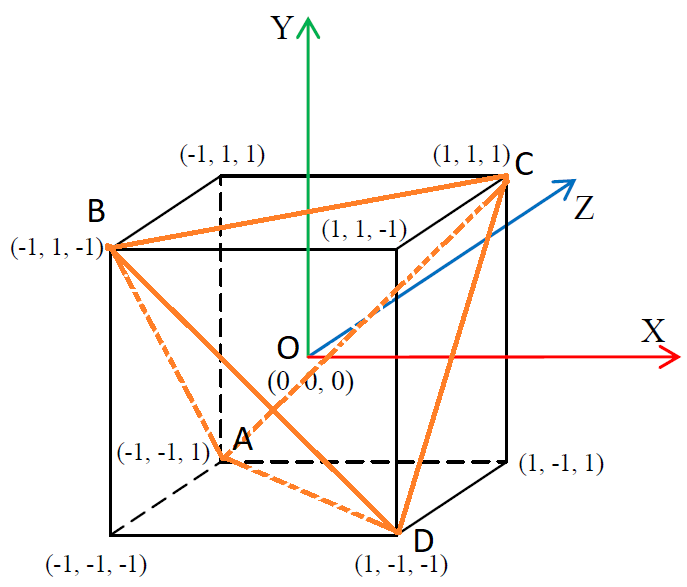
\includegraphics[width=100px]{cube}
    \newline
    \[\overline{|BC|}=(c_{1}-b_{1};c_{2}-b_{2};c_{3}-b_{3})=(2;0;2)\]  \newline
    $ l=\overline{|BC|}=\sqrt{x^2 + y^2 + z^2}=2\sqrt{2}\ $ \newline
    \textrm{BC equals to the diagonal of the square, and since all faces of the cube are equal squares, so their diagonals are equal too.} \newline
    \textrm{b).} \newline
    \textrm{The angle between H and C is equal to the angle between the vectors }$ \overline{OB} $\textrm{ and } $\overline{OC} \textrm{ :} $ \newline
    $ \angle \alpha = \arccos(\frac {\overline{OB}\cdot \overline{OC}} {|\overline{OB}| |\overline{OC}|}) = 121 $ \degree  \newline
    \textrm{c).} \newline
    $\angle (CBD) = \arccos(\frac {\overline{BC}\cdot \overline{BD}}{|\overline{BC}| |\overline{BD}|}) = 60 \degree \newline $
    $\angle \beta = \arccos(\frac {\overline{AB}\cdot \overline{DC}}{|\overline{AB}| |\overline{DC}|}) = 90 \degree \newline $
    \textrm{d).} \newline
    $ S = \frac{BC^2\cdot\sqrt{3}}{4} = 2\sqrt{3} \newline $



    \begin{center}
        \textrm{Problem 2} %error
    \end{center}
    \newline
    \textrm{a).} \newline
    $\overline{v_1}\cdot(\overline{v_2}-\overline{v_3})=0 \newline $
    \textrm{b-c).} \newline
    $\overline{v_1}\cdot\overline{v_2}=\overline{v_1}\cdot\overline{v_3}=\overline{v_2}\cdot\overline{v_3} \newline$
    =>$ \overline{v_1}=\overline{v_2}=\overline{v_3} => \triangle\ $ \textrm{ is equilateral and }$ P$ \textrm{ is also on the altitude from } \[P_3\]

    \begin{center}
        \textrm{Problem 3}
    \end{center}
    \newline
    $\overline{a}\times\overline{b}=\overline{v_1} \newline
    \overline{c}\times\overline{a}=\overline{v_2} \newline
    \overline{b}\times\overline{c}=\overline{v_3} \newline$
    $\overline{v_1}=det(\begin{bmatrix}
                           \overline{i} & \overline{j} & \overline{k}\\
                           a_1 & a_2 & a_3 \\
                           b_1 & b_2 & b_3
    \end{bmatrix}) = \overline{i}\cdot(a_2b_3 - a_3b_2)-\overline{j}\cdot(a_1b_3 - a_3b_1) + \overline{k} \cdot(a_1b_2-a_2b_1) \newline
    \overline{v_2}=det(\begin{bmatrix}
                           \overline{i} & \overline{j} & \overline{k}\\
                           c_1 & c_2 & c_3 \\
                           a_1 & a_2 & a_3
    \end{bmatrix}) = \overline{i}\cdot(c_2a_3 - c_3a_2)-\overline{j}\cdot(c_1a_3 - c_3a_1) + \overline{k} \cdot(c_1a_2-c_2a_1) \newline
    \overline{v_3}=det(\begin{bmatrix}
                           \overline{i} & \overline{j} & \overline{k}\\
                           b_1 & b_2 & b_3 \\
                           c_1 & c_2 & c_3
    \end{bmatrix}) = \overline{i}\cdot(b_2c_3 - b_3c_2)-\overline{j}\cdot(b_1c_3 - b_3c_1) + \overline{k} \cdot(b_1c_2-b_2c_1) \newline
    \overline{v_4}=det(\begin{bmatrix}
                           \overline{i} & \overline{j} & \overline{k}\\
                           (\overline{b}-\overline{c})_1 & (\overline{b}-\overline{c})_2 & (\overline{b}-\overline{c})_3 \\
                           (\overline{a}-\overline{c})_1 & (\overline{a}-\overline{c})_2 & (\overline{a}-\overline{c})_3
    \end{bmatrix}) = \overline{i}\cdot((\overline{b}-\overline{c})_2(\overline{a}-\overline{c})_3 - (\overline{b}-\overline{c})_3(\overline{a}-\overline{c})_2)-\overline{j}\cdot((\overline{b}-\overline{c})_1(\overline{a}-\overline{c})_3 - (\overline{b}-\overline{c})_3(\overline{a}-\overline{c})_1) + \overline{k} \cdot((\overline{b}-\overline{c})_1(\overline{a}-\overline{c})_2-(\overline{b}-\overline{c})_2(\overline{a}-\overline{c})_1) = \overline{i}\cdot(b_2a_3-b_2c_3-c_2a_3+c_2c_3-b_3a_2+b_3c_2+c_3a_2-c_2c_3)+\overline{j}\cdot(b_1a_3-b_1c_3-c_1a_3+c_1c_3-b_3a_1+b_3c_1+c_3a_1-c_1c_3)+\overline{k}\cdot(b_1a_2-a_2c_1-c_2b_1+c_2c_1-b_2a_1+b_2c_1+c_2a_1-c_2c_1) \newline
    \overline{v_1}+\overline{v_2}+\overline{v_3}+\overline{v_4}=\overline{i}\cdot(a_2b_3 - a_3b_2+c_2a_3 - c_3a_2+b_2c_3 - b_3c_2+b_2a_3-b_2c_3-c_2a_3-b_3a_2+b_3c_2+c_3a_2)+\overline{j}\cdot(a_1b_3 - a_3b_1+c_1a_3 - c_3a_1+b_1c_3 - b_3c_1+b_1a_3-b_1c_3-c_1a_3+c_1c_3-b_3a_1+b_3c_1+c_3a_1-c_1c_3)+\overline{k}\cdot(a_1b_2-a_2b_1+c_1a_2-c_2a_1+b_1c_2-b_2c_1+b_1a_2-a_2c_1-c_2b_1+c_2c_1-b_2a_1+b_2c_1+c_2a_1-c_2c_1)=0  \newline
$
    \begin{center}
        \textrm{Problem 4}
    \end{center}
    \textrm{a).} \newline
    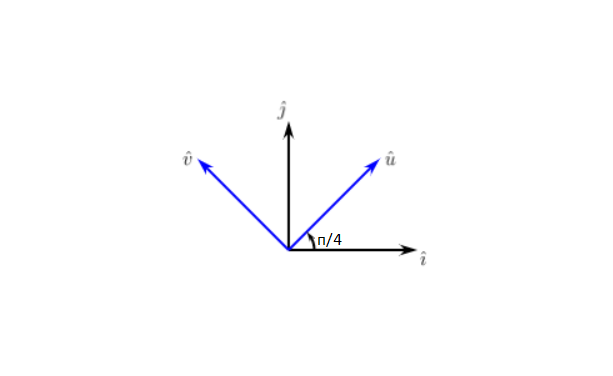
\includegraphics[width=100px]{coord1}
    \newline
    $ A=\begin{bmatrix}
            \frac{\sqrt{2}}{2} & -\frac{\sqrt{2}}{2} \\
            \frac{\sqrt{2}}{2} & \frac{\sqrt{2}}{2}
    \end{bmatrix} \newline
    \overline{v}=A \begin{bmatrix}
                       0\\
                       1
    \end{bmatrix} = \begin{bmatrix}
                        -0.7\\
                        0.7
    \end{bmatrix} \newline
    \overline{u}=A \begin{bmatrix}
                       1\\
                       0
    \end{bmatrix} = \begin{bmatrix}
                        0.7\\
                        0.7
    \end{bmatrix} \newline
    \textrm{b).} \newline
    \begin{bmatrix}
        \cos(\alpha) & -\sin(\alpha)\\
        \sin(\alpha) & \cos(\alpha)
    \end{bmatrix} \times \begin{bmatrix}
                             \cos(\beta) & -\sin(\beta)\\
                             \sin(\beta) & \cos(\beta)
    \end{bmatrix} = \begin{bmatrix}
                        \cos(\alpha)\cdot\cos(\beta)-\sin(\alpha)\cdot\sin(\beta) & -\cos(\alpha)\cdot\sin(\beta)-\sin(\alpha)\cdot\cos(\beta)\\
                        \sin(\alpha)\cdot\sin(\beta)+\cos(\alpha)\cdot\cos(\beta) & \cos(\alpha)\cdot\cos(\beta)-\sin(\alpha)\cdot\sin(\beta)
    \end{bmatrix} = \begin{bmatrix}
                        \cos(\alpha+\beta) & -\sin(\alpha+\beta)\\
                        \sin(\alpha+\beta) & \cos(\alpha+\beta)
    \end{bmatrix} \newline
    \textrm{c).} \newline
    \ d=det(\begin{bmatrix}
                \cos(\alpha) & -\sin(\alpha)\\
                \sin(\alpha) & \cos(\alpha)
    \end{bmatrix}) = \cos(\alpha)^2+\sin(\alpha)^2=1 \newline
    \ M_*=(\begin{bmatrix}
               \cos(\alpha)  & \sin(\alpha)\\
               -\sin(\alpha) & \cos(\alpha)
    \end{bmatrix}) \newline
    \ A^{-1}=\frac{1}{d}\cdot M_*=M_* \newline
    \textrm{1).} \begin{bmatrix}
                     \cos(\alpha)  & \sin(\alpha)\\
                     -\sin(\alpha) & \cos(\alpha)
    \end{bmatrix} \times \begin{bmatrix}
                             \cos(\alpha)  & -\sin(\alpha)\\
                             \sin(\alpha) & \cos(\alpha)
    \end{bmatrix} = \begin{bmatrix}
                        1 & 0\\
                        0 & 1
    \end{bmatrix} = I \newline
    \textrm{2).} \begin{bmatrix}
                     \cos(-\alpha)  & -\sin(-\alpha)\\
                     \sin(-\alpha)  &  \cos(-\alpha)
    \end{bmatrix} = \begin{bmatrix}
                        \cos(\alpha)  & \sin(\alpha)\\
                        -\sin(\alpha) & \cos(\alpha)
    \end{bmatrix} \newline
    \ => A_\theta^{-1}=A_{-\theta} \newline

    \textrm{d).} \newline
    \textrm{1).} \begin{bmatrix}
                     -\frac{\sqrt{2}}{2} & -\frac{\sqrt{2}}{2} \\
                     \frac{\sqrt{2}}{2}  & -\frac{\sqrt{2}}{2}
    \end{bmatrix} \newline
    \textrm{2).} \begin{bmatrix}
                     -\frac{\sqrt{2}}{2} & -\frac{\sqrt{2}}{2} \\
                     -\frac{\sqrt{2}}{2} &  \frac{\sqrt{2}}{2}
    \end{bmatrix} \newline
    \textrm{3).} \begin{bmatrix}
                     -\frac{\sqrt{2}}{2} &  \frac{\sqrt{2}}{2} \\
                     -\frac{\sqrt{2}}{2} & -\frac{\sqrt{2}}{2}
    \end{bmatrix} \newline
    \textrm{4).} \begin{bmatrix}
                     -\frac{\sqrt{2}}{2} & \frac{\sqrt{2}}{2} \\
                     \frac{\sqrt{2}}{2}  & \frac{\sqrt{2}}{2}
    \end{bmatrix} \newline

    \textrm{e).} \newline
    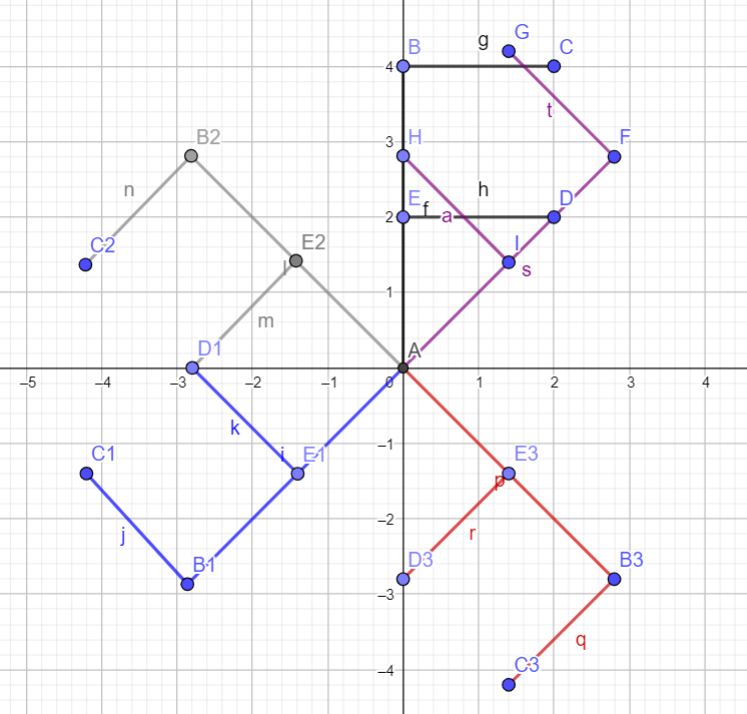
\includegraphics[width=100px]{coord2} \newline

    \begin{center}
        \textrm{Problem 5}
    \end{center}
    \textrm{a). It corresponds to the total number of ingredients in the food assortment.} \newline
    \textrm{b).} \newline
    \ MXN = \begin{bmatrix}
                22x_1 & 40x_2 & 50x_3\\
                18x_1 & 10x_2 & 3 x_3\\
                5 x_1 & 14x_2 & 5 x_3\\
                10x_1 & 10x_2 & 22x_3\\
    \end{bmatrix} \times \begin{bmatrix}
                             0.1  & 0 & 0.13 & 0\\
                             0.76 & 1 & 0.01 & 0\\
                             0.01 & 0 & 0.1  & 82
    \end{bmatrix} \newline
    \textrm{c).} \newline $




\end{document}